\documentclass{beamer}

% used Commands for installing everything needed + VSCode Packages

% sudo apt install texlive-latex-extra
% sudo apt -y install texlive-lang-german
% sudo apt install chktex
% sudo apt install latexmk

% https://hartwork.org/beamer-theme-matrix/

%Style
\mode<presentation>{
    %Theme
    %\usetheme{default}
    %\usetheme{AnnArbor}
    %\usetheme{Antibes}
    %\usetheme{Bergen}
    %\usetheme{Berkeley}
    %\usetheme{Berlin}
    %\usetheme{Boadilla}
    %\usetheme{CambridgeUS}
    %\usetheme{Copenhagen}      ||||||
    %\usetheme{Darmstadt}
    %\usetheme{Dresden}
    %\usetheme{Frankfurt}
    %\usetheme{Goettingen}
    %\usetheme{Hannover}
    %\usetheme{Ilmenau}
    %\usetheme{JuanLesPins}
    %\usetheme{Luebeck}
    %\usetheme{Madrid}
    %\usetheme{Malmoe}           ||||||||||||||
    %\usetheme{Marburg}
    %\usetheme{Montpellier}
    %\usetheme{PaloAlto}
    %\usetheme{Pittsburgh}
    %\usetheme{Rochester}
    %\usetheme{Singapore}
    %\usetheme{Szeged}
    %\usetheme{Warsaw}
    %\usetheme{metropolis}                          ||||||||||||||||||||||||||||||||
    
    %Farb-Theme
    %\usecolortheme{albatross}
    %\usecolortheme{beaver}             ||||||||||||||||||||||||||||
    %\usecolortheme{beetle}
    %\usecolortheme{crane}
    %\usecolortheme{dolphin}      |||||||
    %\usecolortheme{dove}
    %\usecolortheme{fly}
    %\usecolortheme{lily}
    %\usecolortheme{orchid}
    %\usecolortheme{rose}
    %\usecolortheme{seagull}
    %\usecolortheme{seahorse}
    %\usecolortheme{whale}
    %\usecolortheme{wolverine}

    %\setbeamertemplate{footline} % Fußzeile entfernen
    %\setbeamertemplate{footline}[page number] % Fußzeile entfernen und durch Folien-Zahl ersetzen

    %\setbeamertemplate{navigation symbols}{} % Navigations-Symbole entfernen
}

%Packages
\usepackage[utf8]{inputenc} %Deutsche Umlaute
\usepackage[ngerman]{babel} %Deutsche Sprache
\usepackage{graphicx}       %für Bilder
\usepackage{booktabs}       %für \toprule \midrule \bottomrule in Tabellen


%Einstellungen der Präsi
\title{Speedcubing}
\author{Kimi Löffel}
\institute[Bbc]{ICT Berufsbildungscenter}
\date{\today}



\begin{document}

    %Titelseite
    \begin{frame}
        \titlepage{}
        \end{frame}



    %Inhaltsverzeichnis
    \begin{frame}{Inhalt}
        \tableofcontents
    \end{frame}



    \section{What is it?}


        %What is Speedcubing
        \begin{frame}{What is it?}
            \begin{itemize}
                \item Speedsolving a puzzle \pause{}
                \item Collecting Puzzles \pause{}
                \item Modders
            \end{itemize}
        \end{frame}
    


    \section{Puzzles}
        \subsection{WCA}
        
            \subsubsection{What is the WCA?}



                %What is the WCA
                \begin{frame}{What is the WCA}
                    \begin{itemize}
                        \item World Cube Association \pause{}
                        \item Organizes Competitions \pause{}
                        \item Award official records
                    \end{itemize}
                \end{frame}

            \subsubsection{WCA puzzles/events}

                %All WCA puzzles and events
                \begin{frame}{WCA puzzles and events}
                    \begin{columns}[c] 
                        \column{.27\textwidth} %linke spalte
                            \begin{itemize}
                                \item 3$\times$3$\times$3 \pause{}
                                \item 2$\times$2$\times$2 \pause{}
                                \item 4$\times$4$\times$4 \pause{}
                                \item 5$\times$5$\times$5 \pause{}
                                \item 6$\times$6$\times$6 \pause{}
                                \item 7$\times$7$\times$7 \pause{}
                                \item 3$\times$3$\times$3 BLD \pause{}
                                \item 3$\times$3$\times$3 FMC \pause{}
                                \item 3$\times$3$\times$3 OH \pause{}
                            \end{itemize}
                        \column{.3\textwidth} % mittlere Spalte
                            \begin{itemize}
                                \item Clock \pause{}
                                \item Megaminx \pause{}
                                \item Pyraminx \pause{}
                                \item Skewb \pause{}
                                \item Square-1 \pause{}
                                \item 4$\times$4$\times$4 BLD \pause{}
                                \item 5$\times$5$\times$5 BLD \pause{}
                                \item 3$\times$3$\times$3 Multi-BLD \pause{}
                            \end{itemize}
                        \column{.25\textwidth} %rechte spalte 1

                            \begin{figure}
                                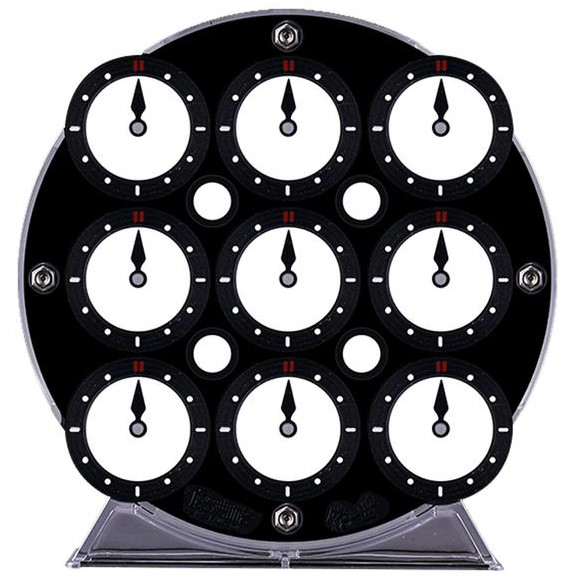
\includegraphics[width=0.6\textwidth]{assets/clock.jpg} \pause{}
                            \end{figure}

                            \begin{figure}
                                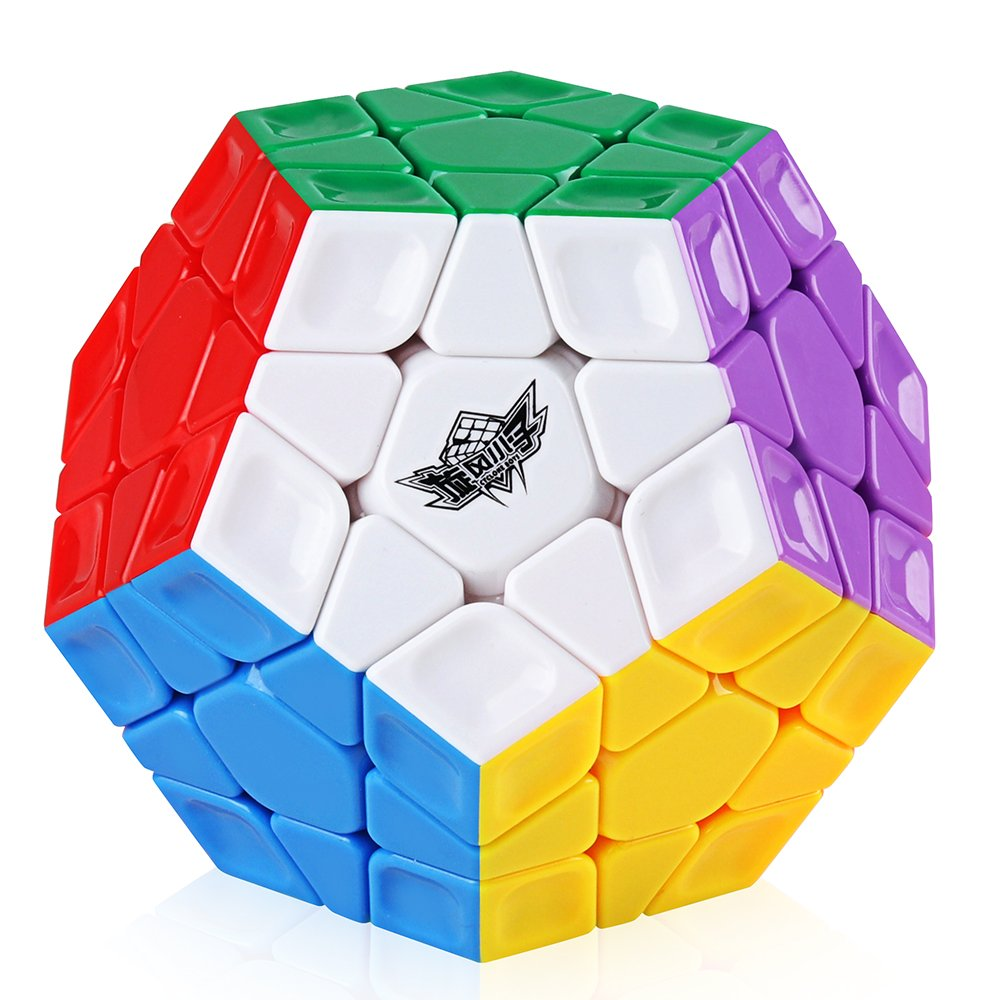
\includegraphics[width=0.6\textwidth]{assets/mega.jpg} \pause{}
                            \end{figure}

                            \begin{figure}
                                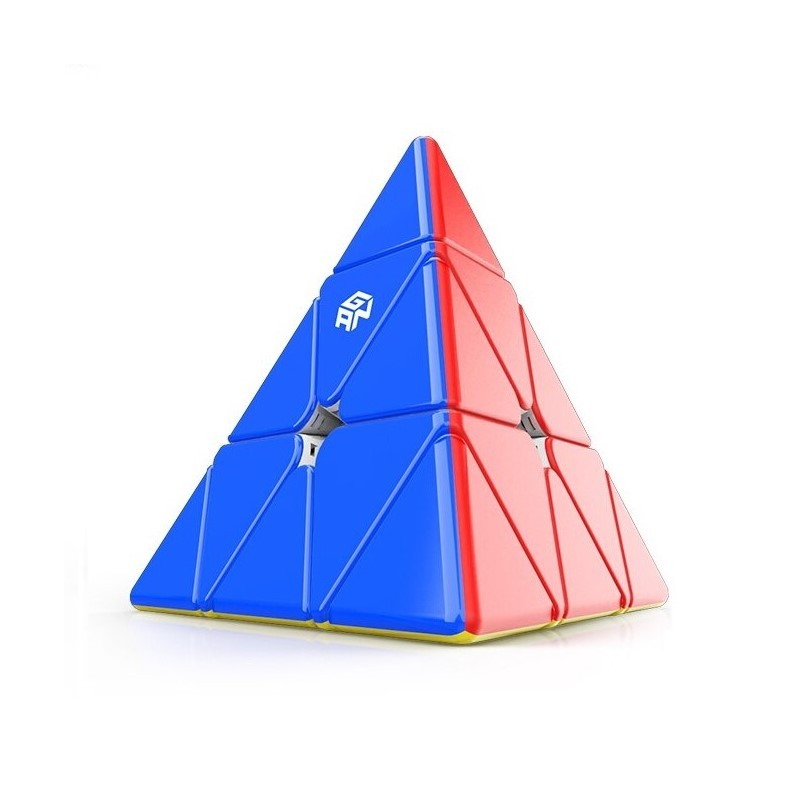
\includegraphics[width=0.7\textwidth]{assets/pyra.jpg} \pause{}
                            \end{figure}

                        \column{.25\textwidth} %rechte spalte 2

                            \begin{figure}
                                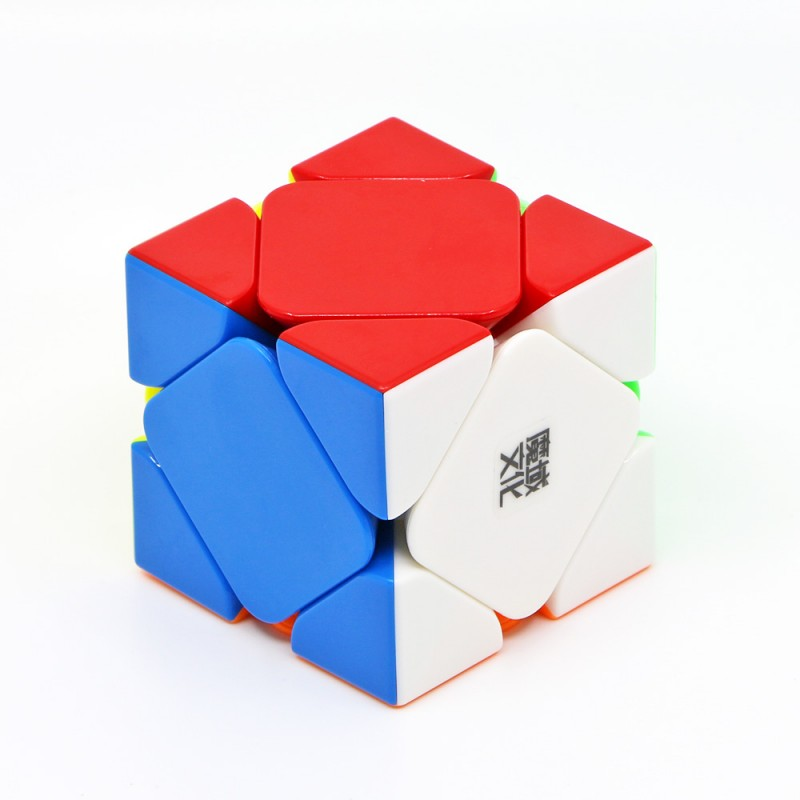
\includegraphics[width=0.9\textwidth]{assets/skewb.jpg} \pause{}
                            \end{figure}

                            \begin{figure}
                                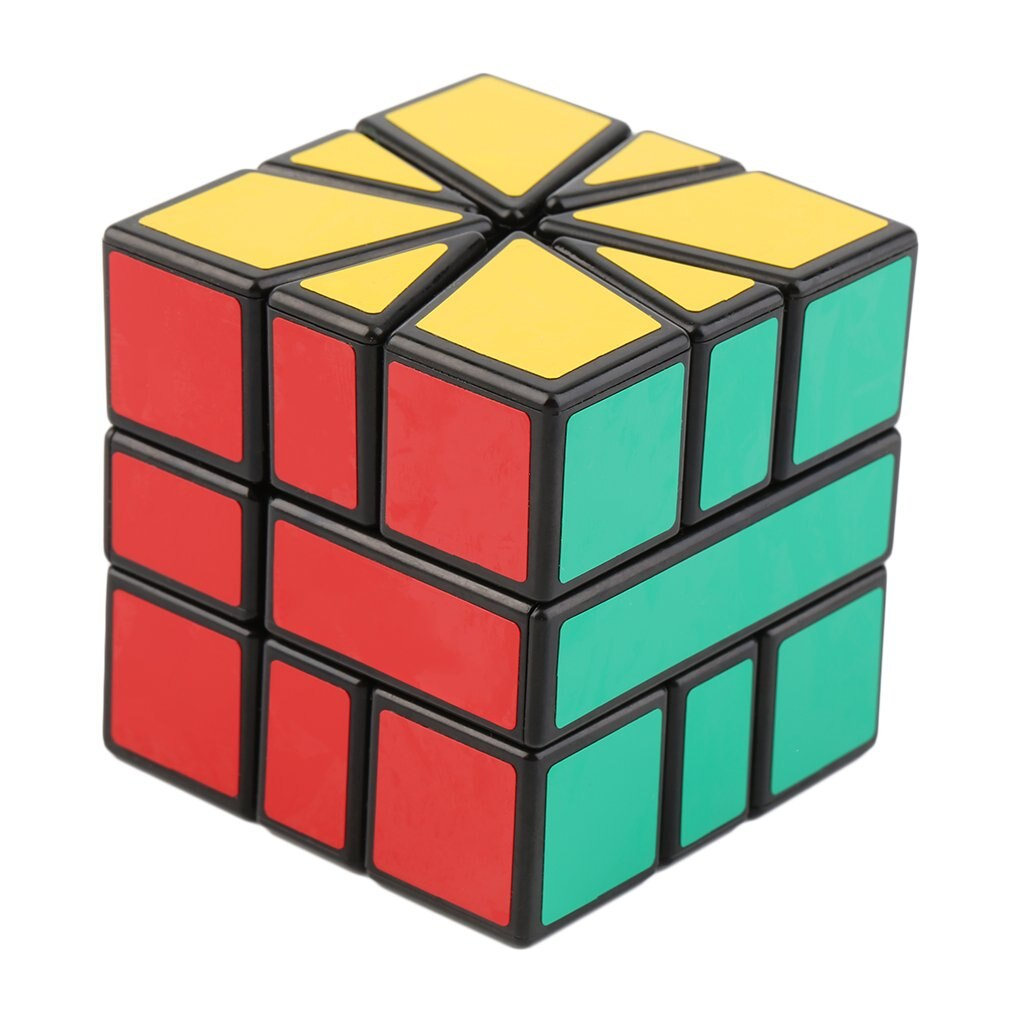
\includegraphics[width=0.8\textwidth]{assets/square1.jpg} \pause{}
                            \end{figure}
                    \end{columns}
                \end{frame}

        \subsection{non WCA}
            \begin{frame}{non WCA puzzles}
                \begin{figure}
                    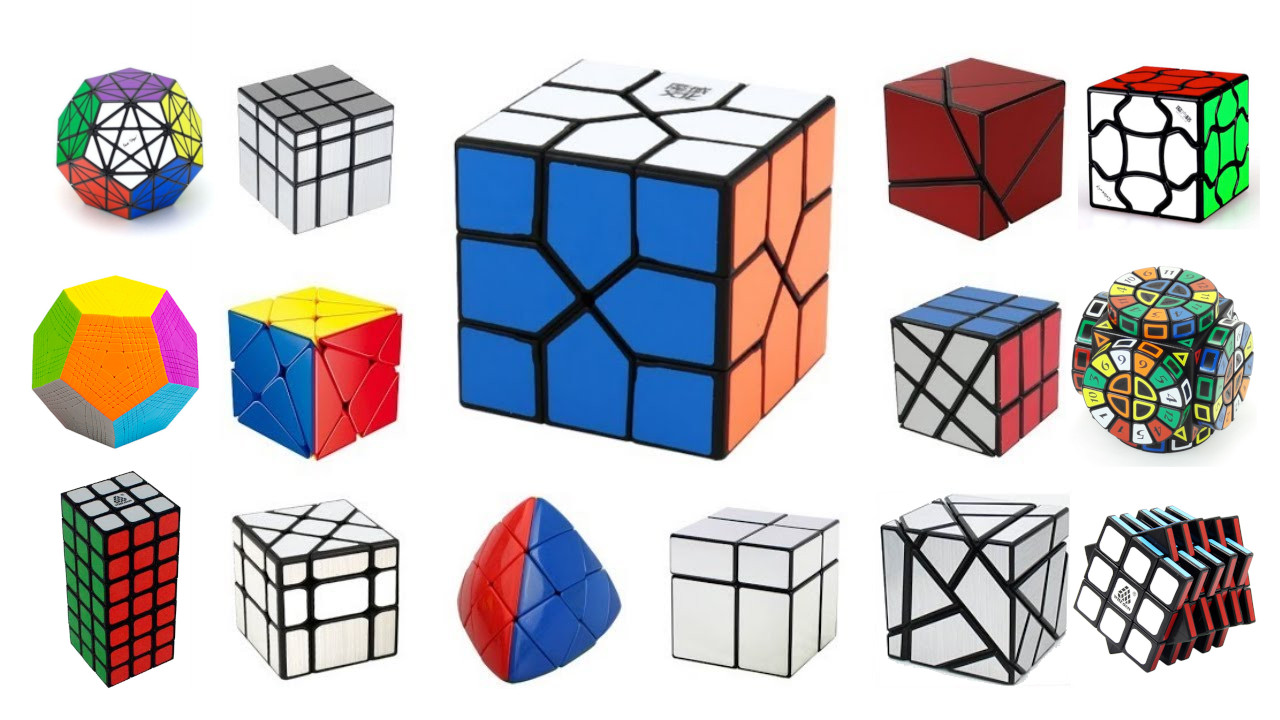
\includegraphics[width=\textwidth]{assets/nonWCAall.jpg}
                \end{figure}
            \end{frame}
        \subsection{Shops}
            \begin{frame}{Cube-Shops}
                \begin{itemize}
                    \item Fabitasia
                    \item Cubeshop Schweiz
                    \item Cubeless
                    \item EuroCubes
                    \item Cubicle
                    \item Speedcubeshop
                \end{itemize}
            \end{frame}
        
    \section{Solving methods}
        \subsection{Beginners}
            \begin{frame}{Beginners method}
                \begin{itemize}
                    \item Cross $\rightarrow{}$ First Layer $\rightarrow{}$ First two layers $\rightarrow{}$ Orient edges of LL $\rightarrow{}$ Permute edges of LL $\rightarrow{}$ Permute edges of LL $\rightarrow{}$ Orient edges of LL \pause{} 
                    \item Slow $\rightarrow{}$ not meant for speedsolving \pause{}
                    \item Easy to learn
                \end{itemize}
            \end{frame}
        \subsection{CFOP}
            \begin{frame}{CFOP method}
                \begin{itemize}
                    \item Cross $\rightarrow{}$ F2L $\rightarrow{}$ OLL $\rightarrow{}$ PLL \pause{} 
                    \item Used by some of the best speedsolvers in the world \pause{}
                    \item Easy to learn
                \end{itemize}
            \end{frame}
        \subsection{ROUX}
        \begin{frame}{ROUX method}
                \begin{itemize}
                    \item Block $\rightarrow{}$ second Block $\rightarrow{}$ Orient and perumte corners of LL $\rightarrow{}$ Orient last edges$\rightarrow{}$ Permute last edges \pause{} 
                    \item Used by some of the best speedsolvers in the world \pause{}
                    \item Quite intuitive
                \end{itemize}
            \end{frame}
        \subsection{others}
            \begin{frame}{Other methods}
                \begin{itemize}
                    \item Kociemba $\rightarrow{}$ Computer \pause{}
                    \item ZZ $\rightarrow{}$ speedsolving \pause{}
                    \item Petrus $\rightarrow{}$ old speedsolving method \pause{}
                    \item Old Pochmann method $\rightarrow{}$ BLD \pause{}
                    \item 3-Style $\rightarrow{}$ BLD \pause{}
                    \item Variations of each one 
                \end{itemize}
            \end{frame}
    \section{What about me?}
        \begin{frame}{What about me?}
            \begin{itemize}
                \item Started in November 2020 \pause{}
                \item Speedsolver \pause{}
                \item Main events: \pause{}
                \begin{enumerate}
                    \item 3$\times$3$\times$3 \pause{}
                    \item 3$\times$3$\times$3 OH \pause{}
                    \item 2$\times$2$\times$2 \pause{}
                \end{enumerate}
                \item Average around 16 seconds $\rightarrow$ Official Ao5 17.01 \pause{}
                \item PB 10.18s $\rightarrow$ Official PB 12.11\pause{}
                \item WCA ID $\rightarrow$ 2021LOFF01
            \end{itemize}
        \end{frame}
    \begin{frame}{}
        \centering \Large
        \emph{Thank you for listening}
        \end{frame}
\end{document}